\section{Geometric Image Transformations}
\begin{frame}<beamer>
    \frametitle{Outline}
    \tableofcontents[currentsection]
\end{frame}

\begin{frame}
\frametitle {About Basic Geometric Transformations on Image}
\begin{itemize}
	\item {We already know how to process image as a multi-variable function}
	\item {We want to see how image is processed as a geometric matrix/map}
	\item {Basic linear transformations will be covered}
	\begin{itemize}
		\item {Translation}
		\item {Rotation}
		\item {Scaling}
		\item {Affine}
	\end{itemize}
\end{itemize}
\begin{figure}
	{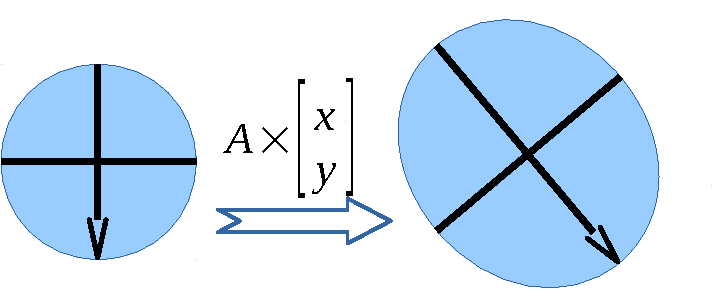
\includegraphics[width=0.5\linewidth]{./figs/imgtrans_demo.pdf}}
\end{figure}
\end{frame}

\begin{frame}
\frametitle {Image Translation}
\begin{itemize}
	\item {Move image along x, y directions or both as a whole}
\end{itemize}
\vspace{0.15in}
\begin{figure}
	{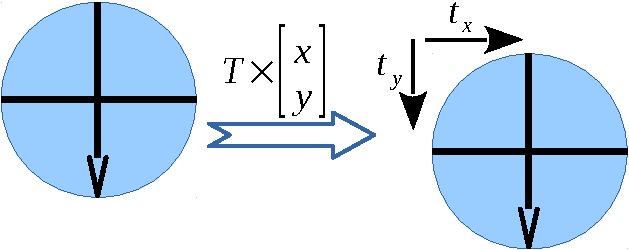
\includegraphics[width=0.6\linewidth]{./figs/imgtrans_trans.pdf}}
\end{figure}
\begin{equation}
	[x'~~y'~~1]^T= \left[ \begin{array}{ccc}
	1 & 0 & t_x \\
	0 & 1 & t_y \\
	0 & 0 & 1 
	\end{array} \right] \left[ \begin{array}{c}
	x \\
	y \\
	1
	\end{array} \right]
\end{equation}
\end{frame}

\begin{frame}
\frametitle {Image Rotation}
\begin{itemize}
	\item {Move image along x, y directions or both as a whole}
\end{itemize}
\vspace{0.1in}
\begin{figure}
	{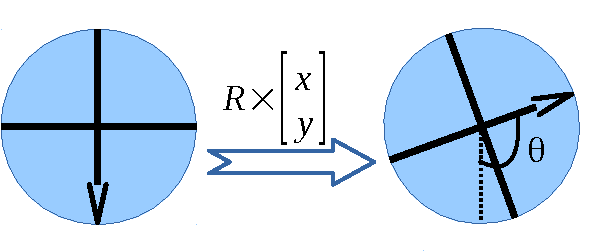
\includegraphics[width=0.6\linewidth]{./figs/imgtrans_rotate.pdf}}
\end{figure}
\begin{equation}
	[x'~~y'~~1]^T=\left[ \begin{array}{ccc}
	cos(\theta) & -sin(\theta) & 0 \\
	sin(\theta) & cos(\theta) & 0 \\
	0 & 0 & 1 
	\end{array} \right] \left[ \begin{array}{c}
	x \\
	y \\
	1
	\end{array} \right]
\end{equation}
\begin{itemize}
	\item {Notice that $R^{-1}=R^{T}$}
\end{itemize}
\end{frame}

\begin{frame}
\frametitle {Image Scaling}
\begin{itemize}
	\item {To achieve zoom-in or zoom-out effect}
\end{itemize}
\vspace{0.1in}
\begin{figure}
	{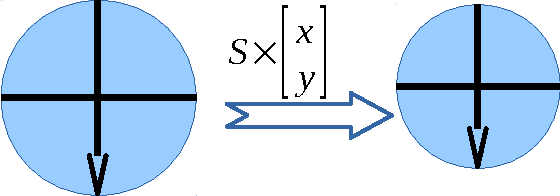
\includegraphics[width=0.6\linewidth]{./figs/imgtrans_scale.pdf}}
\end{figure}
\begin{equation}
	[x'~~y'~~1]^T= \left[ \begin{array}{ccc}
	s_x & 0 & 0 \\
	0 & s_y & 0 \\
	0 & 0 & 1 
	\end{array} \right] \left[ \begin{array}{c}
	x \\
	y \\
	1
	\end{array} \right]
\end{equation}
\begin{itemize}
	\item {Notice that the scaling factors for x and y directions, $s_x$ and $s_y$ could be different}
\end{itemize}
\end{frame}

\begin{frame}
\frametitle {Image Reflection}
\begin{itemize}
	\item {Also known as mirroring}
\end{itemize}
\vspace{0.1in}
\begin{figure}
	{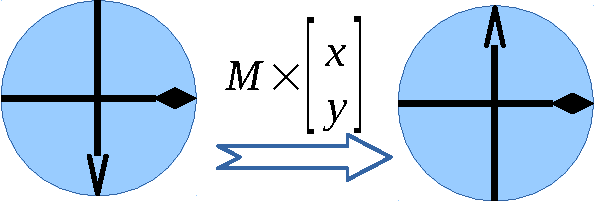
\includegraphics[width=0.55\linewidth]{./figs/imgtrans_mirr.pdf}}
	\hspace{0.15in}
	{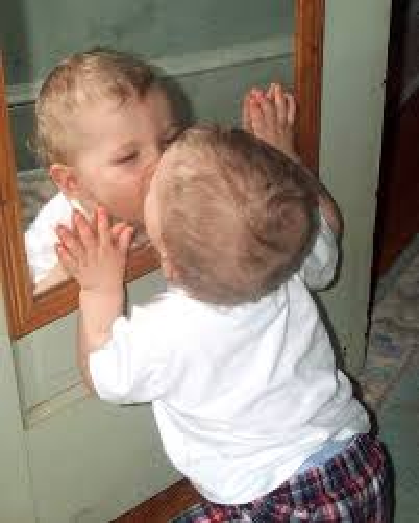
\includegraphics[width=0.15\linewidth]{./figs/mirror.pdf}}
\end{figure}
\begin{equation}
	[x'~~y'~~1]^T=\left[ \begin{array}{ccc}
	1 & 0 & 0 \\
	0 & -1 & 0 \\
	0 & 0 & 1 
	\end{array} \right] \left[ \begin{array}{c}
	x \\
	y \\
	1
	\end{array} \right]
\end{equation}
\begin{itemize}
	\item {You cannot achieve this by rotating}
	\item {If you mirror x and y both, it is then equivalent to rotating 180 degree}
\end{itemize}
\end{frame}

\begin{frame}
\frametitle {Image Affine Transformation}
\begin{itemize}
	\item {There is another one called `shear', check yourself what it is}
	\item {Basic transformations are \textbf{independent} from each other}
\end{itemize}
\vspace{0.1in}
\begin{figure}
	{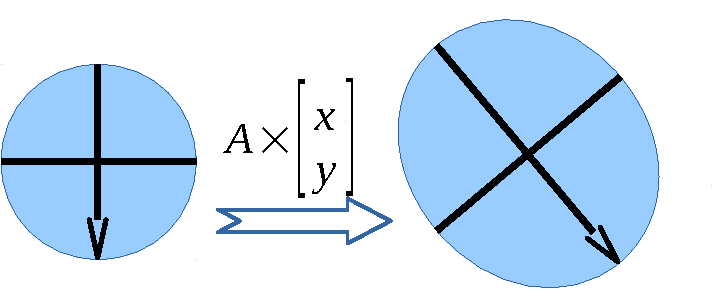
\includegraphics[width=0.6\linewidth]{./figs/imgtrans_demo.pdf}}
\end{figure}
\begin{equation}
	[x'~~y'~~1]^T= T{\cdot}S{\cdot}R{\cdot}M{\cdot}\left[ \begin{array}{c}
	x \\
	y \\
	1
	\end{array} \right]
\end{equation}
\begin{itemize}
	\item {Affine is a combination of these basic transformations}
\end{itemize}
\end{frame}

\begin{frame}
\frametitle {Geometrical Invariance (1)}
\begin{itemize}
	\item {If a vision system still recognizes what the object is after the object is geometrically transformed}
	\item {We say that this vision system is capable of geometrical invariance}
	\item {This is an IMPORTANT concept}
	\item {Our vision system is capable of geometrical invariance in various degree}
\end{itemize}

\end{frame}

\begin{frame}
\frametitle {Geometrical Invariance: rotation invariance (1)}
\begin{itemize}
	\item {How much our vision achieves rotation invariance}
\end{itemize}
\begin{figure}
	{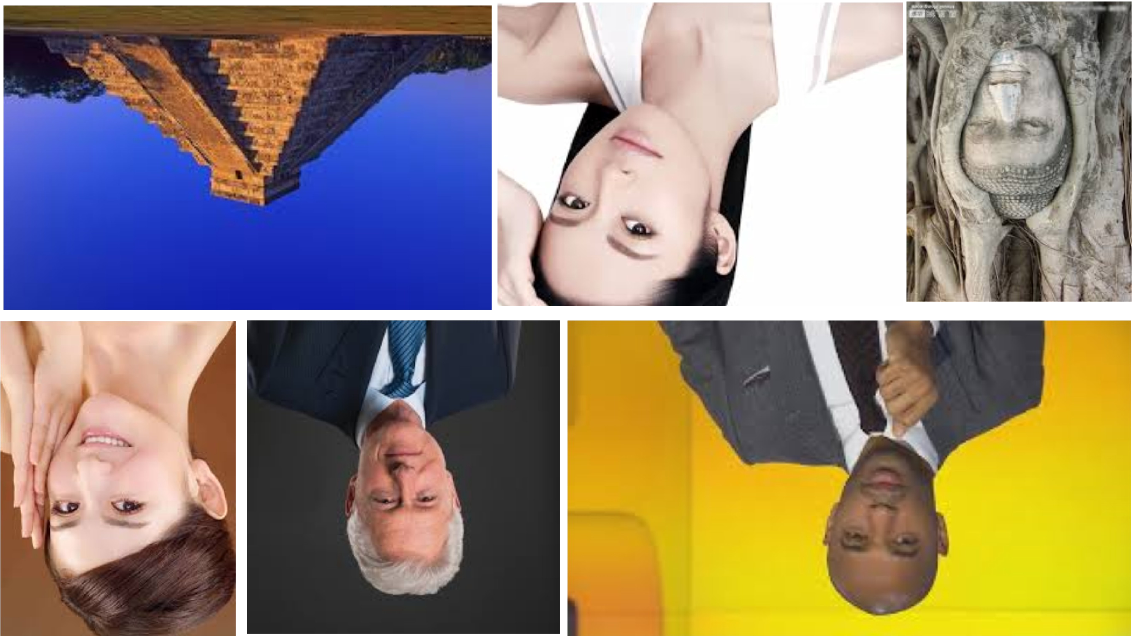
\includegraphics[width=0.75\linewidth]{./figs/invariance_rotate1.pdf}}
\end{figure}
\end{frame}

\begin{frame}
\frametitle {Geometrical Invariance: rotation invariance (2)}
\begin{itemize}
	\item {How much our vision achieves rotation invariance}
\end{itemize}
\begin{figure}
	{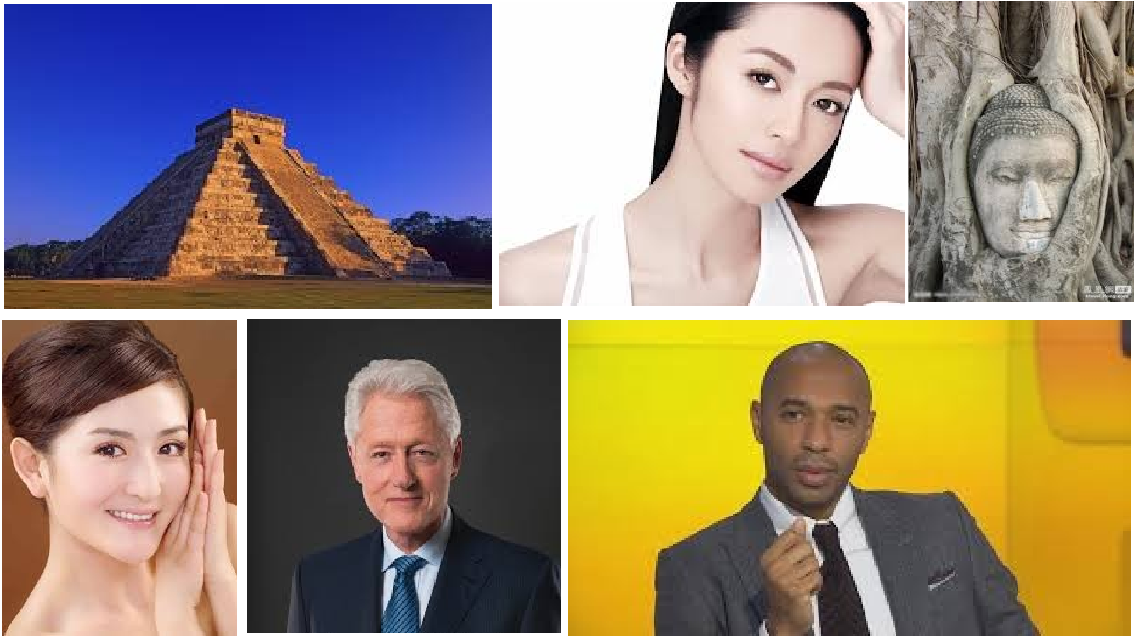
\includegraphics[width=0.75\linewidth]{./figs/invariance_rotate2.pdf}}
\end{figure}
\begin{itemize}
	\item {Verify your answer:)}
\end{itemize}
\end{frame}

\begin{frame}
\frametitle {Geometrical Invariance: scale invariance (1)}
\begin{itemize}
	\item {What you can see from the image?}
\end{itemize}
\begin{figure}
	{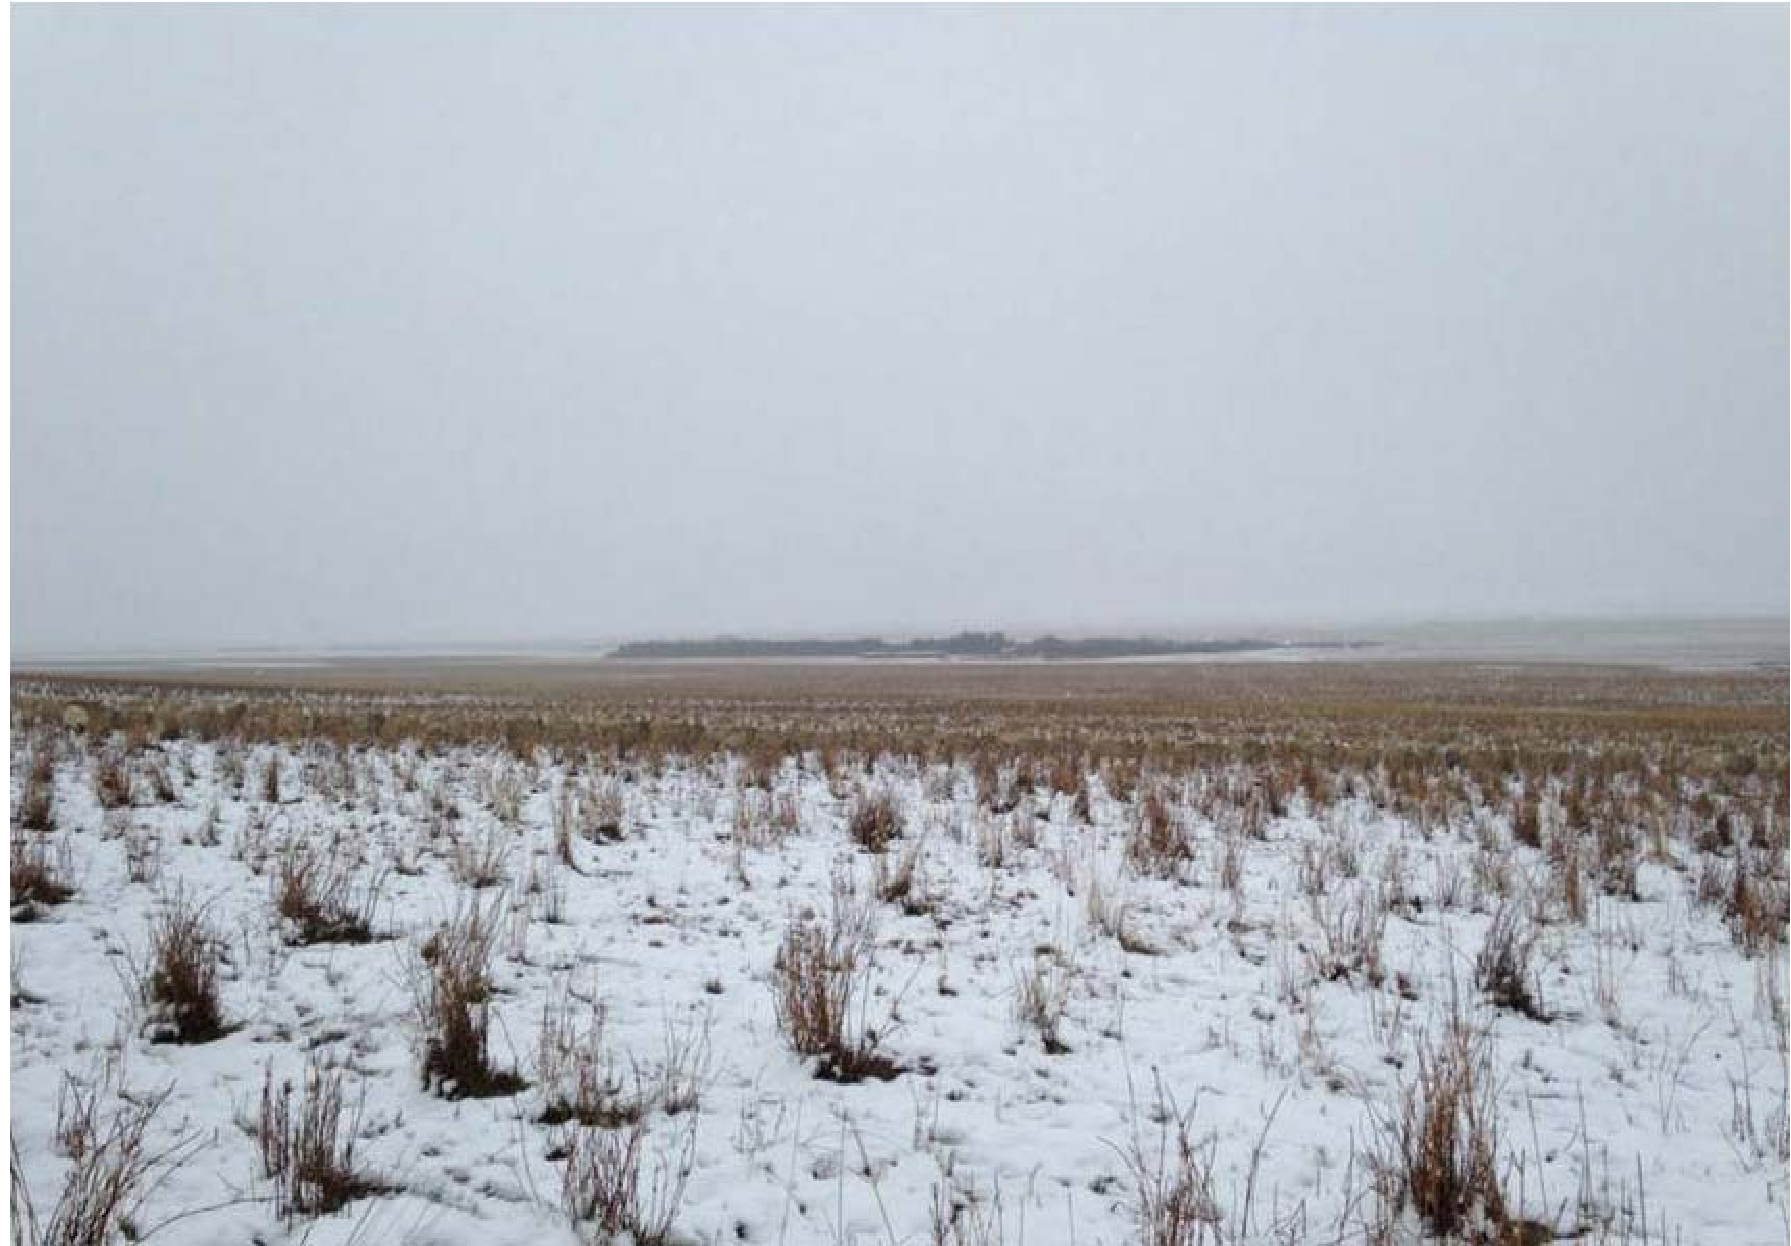
\includegraphics[width=0.7\linewidth]{./figs/scale_sheep1.pdf}}
\end{figure}
\begin{itemize}
	\item {grass, snow and ??}
\end{itemize}
\end{frame}

\begin{frame}
\frametitle {Geometrical Invariance: scale invariance (2)}
\begin{itemize}
	\item {Get closer, what you can see from the image?}
\end{itemize}
\begin{figure}
	{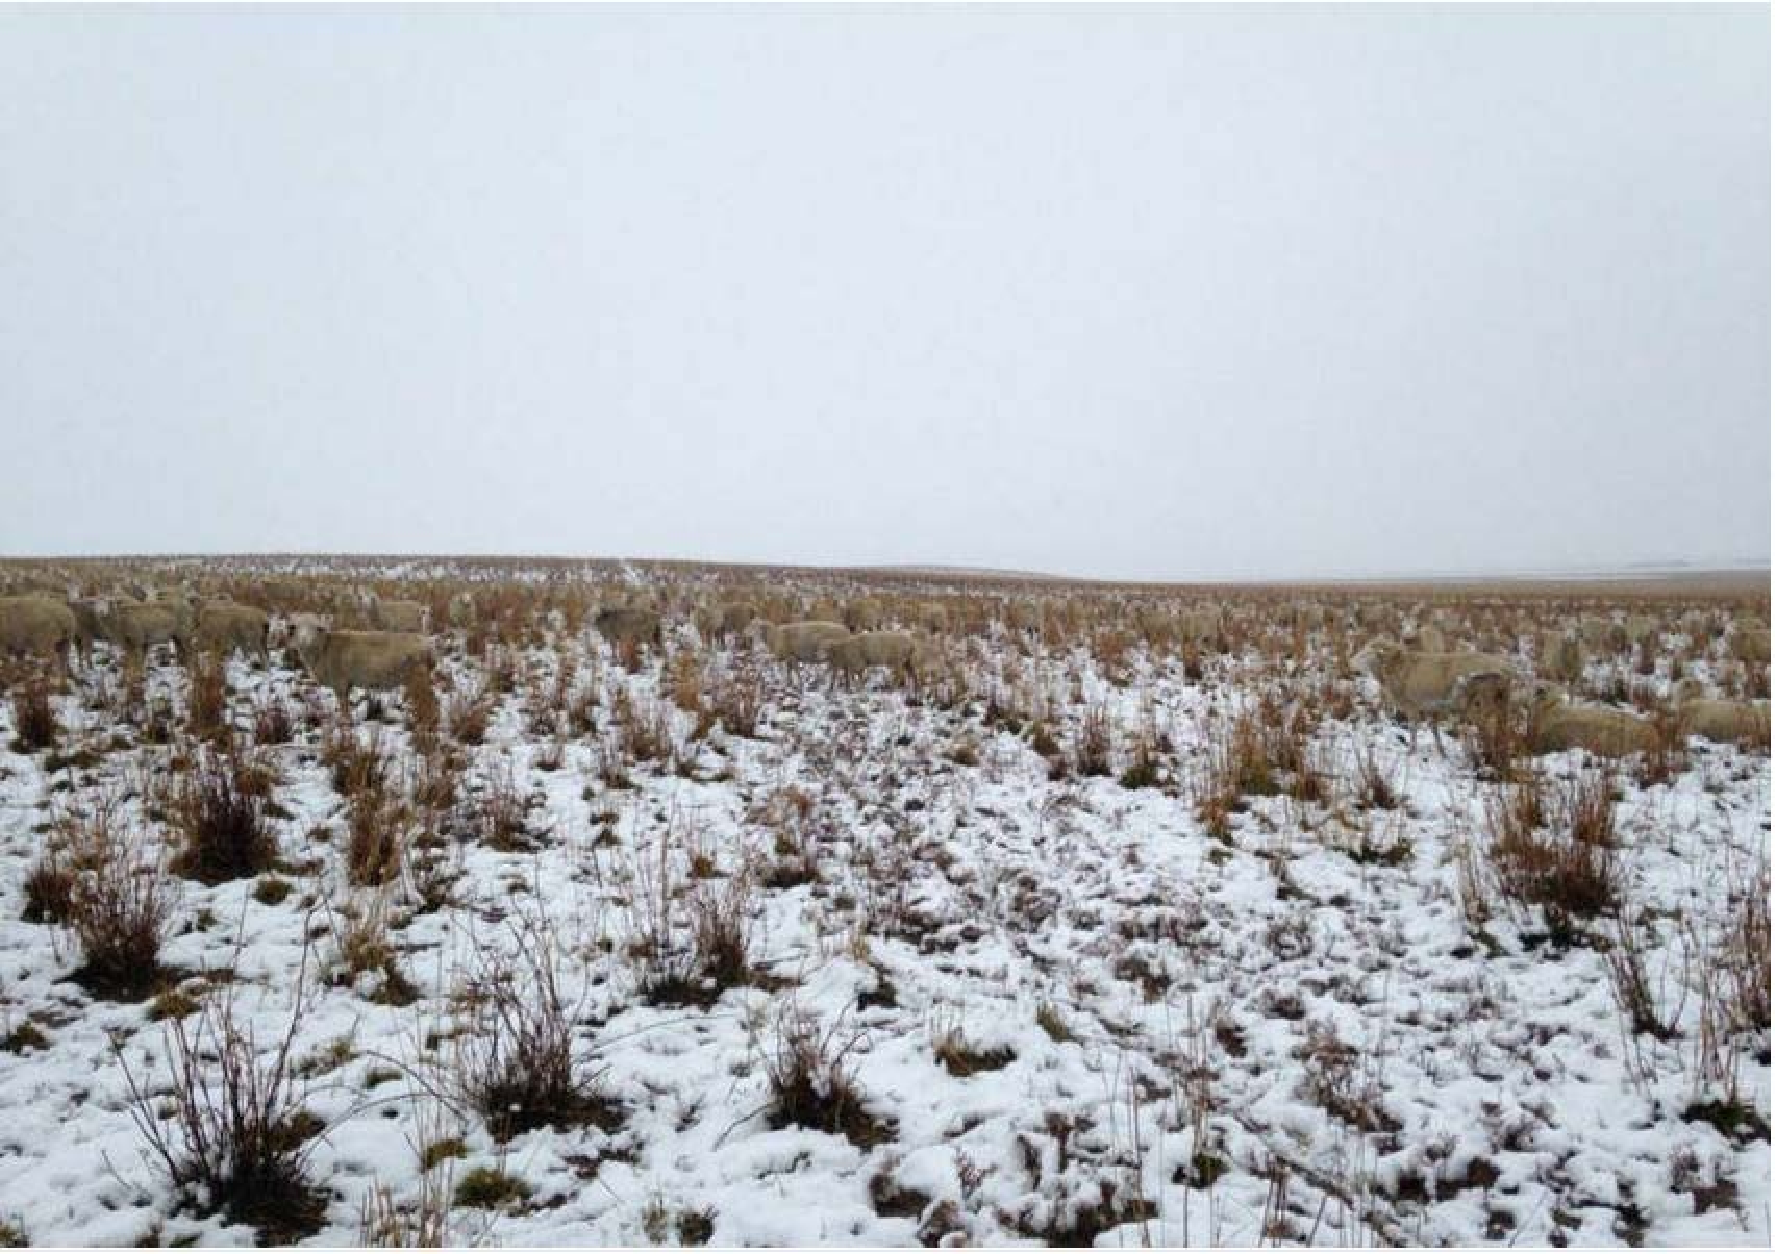
\includegraphics[width=0.65\linewidth]{./figs/scale_sheep2.pdf}}
\end{figure}
\begin{itemize}
	\item {grass, snow and ??}
\end{itemize}
\end{frame}

\begin{frame}
\frametitle {Geometrical Invariance: scale invariance (3)}
\begin{itemize}
	\item {Get closer, what you can see from the image?}
\end{itemize}
\begin{figure}
	{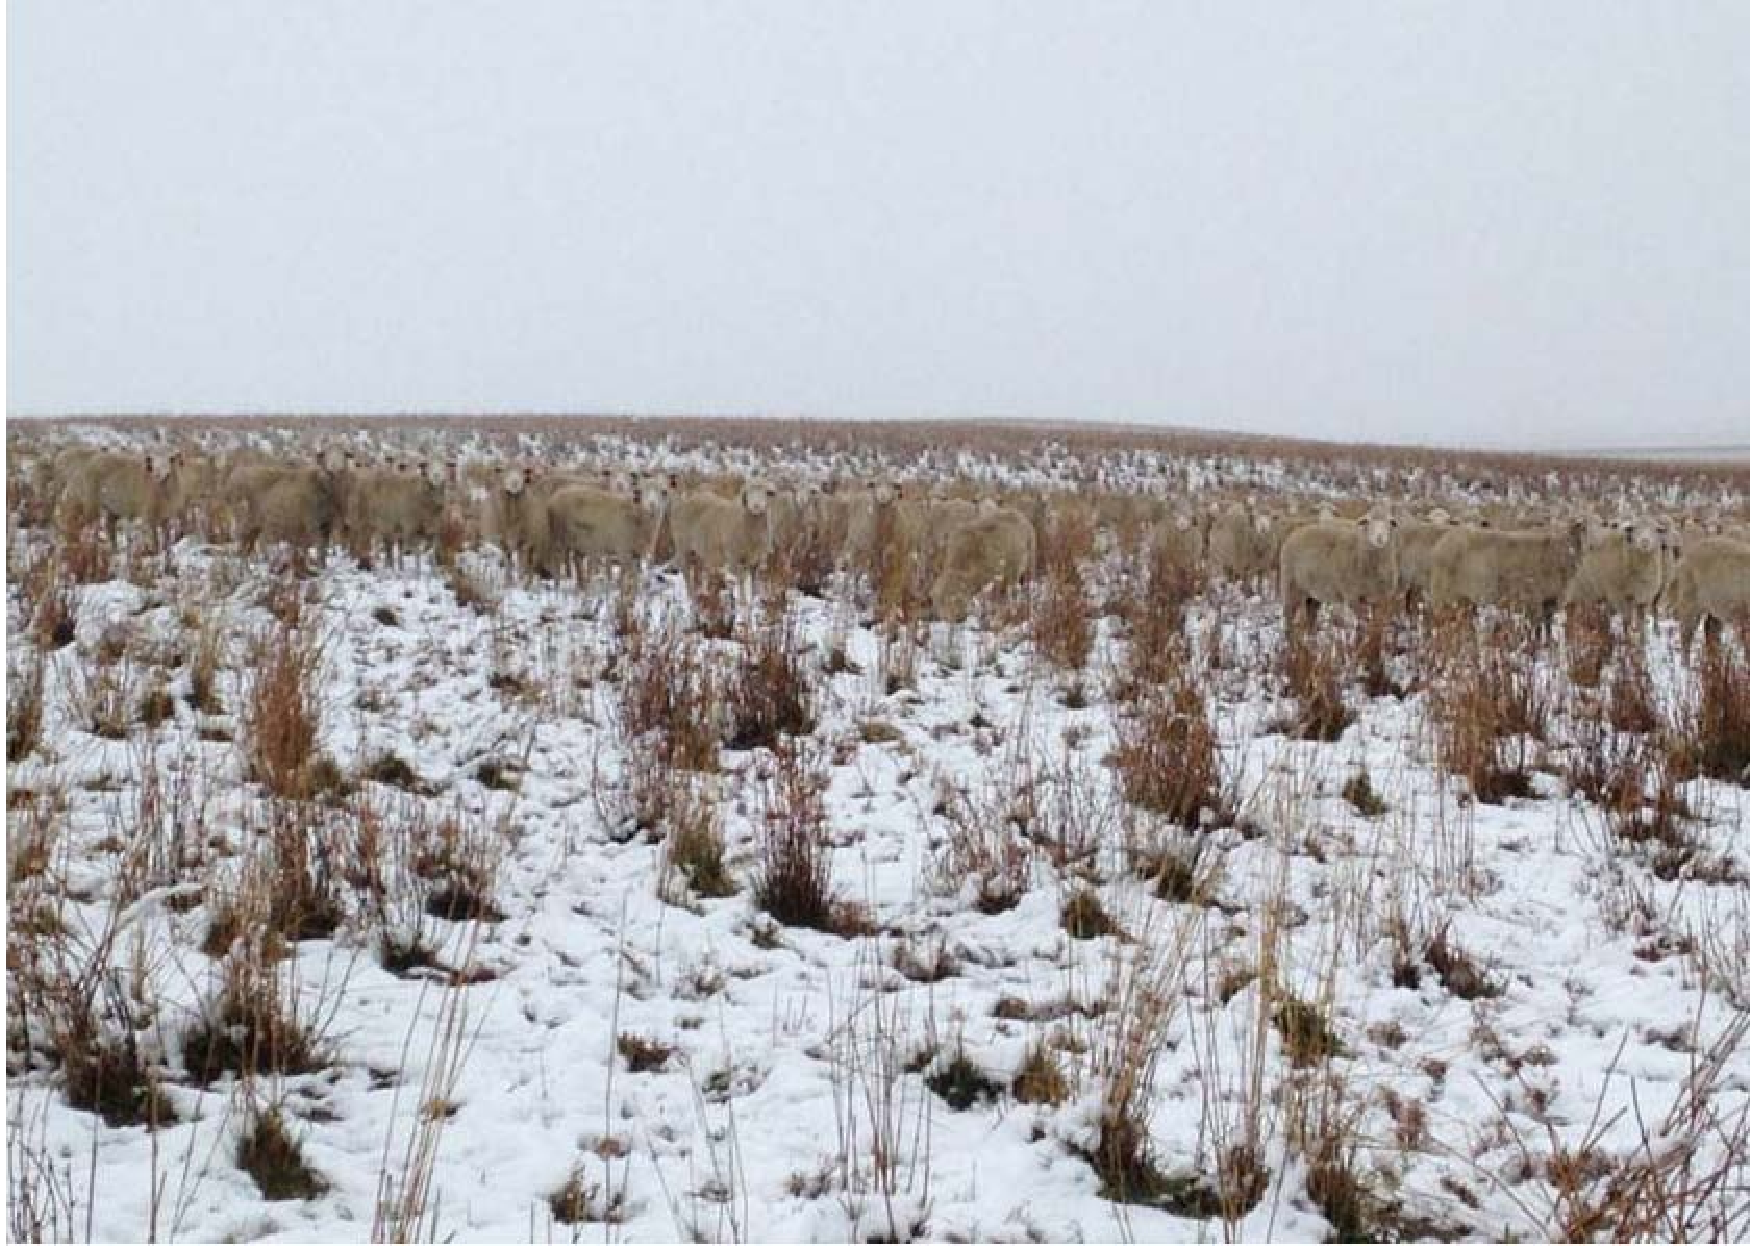
\includegraphics[width=0.65\linewidth]{./figs/scale_sheep3.pdf}}
\end{figure}
\begin{itemize}
	\item {grass, snow and sheep, clearly}
	\item {Conclusion: our vision is partially scale invariant}
\end{itemize}
\end{frame}

\begin{frame}

\frametitle {Geometrical Invariance: affine invariance (1)}
\begin{itemize}
	\item {How much our vision achieves affine invariance}
\end{itemize}
\begin{figure}
	{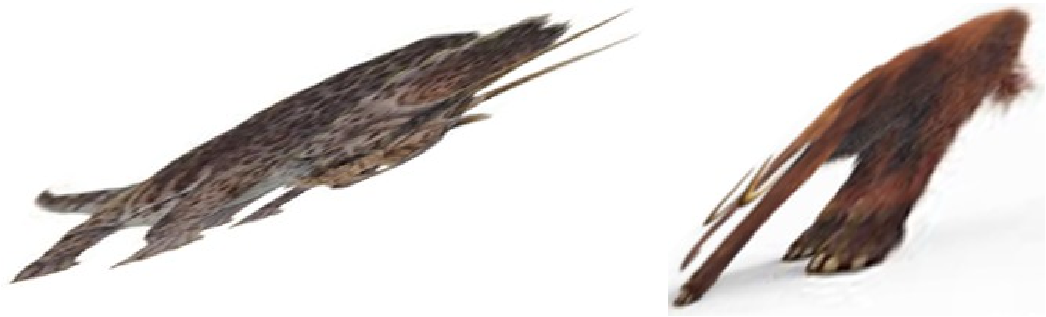
\includegraphics[width=0.75\linewidth]{./figs/invariance_affine1.pdf}}
\end{figure}
\end{frame}

\begin{frame}
\frametitle {Geometrical Invariance: affine invariance (2)}
\begin{itemize}
	\item {How much our vision achieves affine invariance}
\end{itemize}
\begin{figure}
	{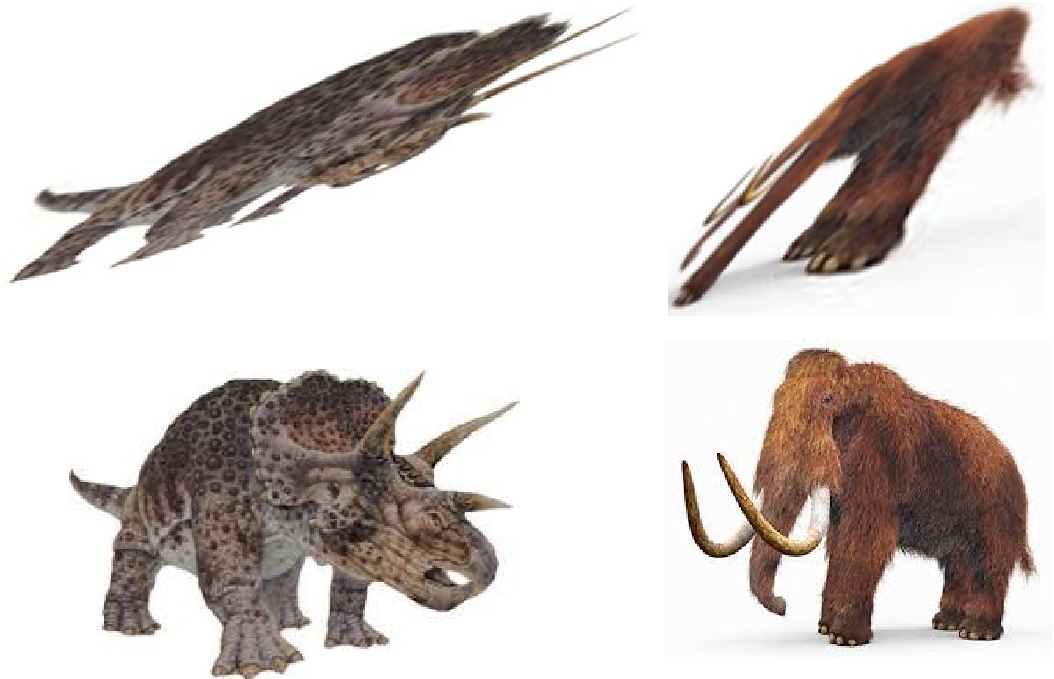
\includegraphics[width=0.75\linewidth]{./figs/invariance_affine2.pdf}}
\end{figure}
\begin{itemize}
	\item {Verify your answer:)}
\end{itemize}
\end{frame}